\documentclass{article}
\usepackage{graphicx} % Required for inserting images
\usepackage{amsmath}
\usepackage{amssymb}
\usepackage[dvipsnames]{xcolor}
\title{SRVAE math}
\author{Etienne Bardet}
\date{May 2025}
\usepackage[backend=biber]{biblatex}
\addbibresource{refs.bib}
\begin{document}

\maketitle

\section{Introduction}
Ce document a pour but de détailler les calculs formulant la loss d'un VAE dans un premier temps puis d'un VAE Conditionnel ("à deux étages") dans un second temps.

\section{VAE}\label{vae}
\subsection{Évidence}
Dans un VAE, nous cherchons à maximiser l'évidence, qui est la probabilité de retrouver notre données, conditionné sur les paramètres du modèle, soit :
\begin{equation*}
    p(x) = \int p(x|z) p(z)dz
\end{equation*}

\subsection{Encodeur}

Cependant, pour estimer $p(x|z)$, il nous faut connaitre $p(z|x)$ pour utiliser le théorème de Bayes.

Nous allons approcher cette distribution par un réseau de neurones qui fournira $q_{\phi}(z|x)$.
Nous supposons ici que la distribution des données de l'espace latent est gaussienne, soit :
\begin{equation*}
    q_{\phi}(z|x) \sim \mathcal{N}(\mu_{\phi}, \Sigma_{\phi})
\end{equation*}
Avec $\Sigma_\phi$ une matrice de covariance diagonale (les $l$ coefficients de sa diagonale étant $l$ sorties de l'encodeur). $\mu_\phi$ étant une autre sortie de l'encodeur, de même taille.

\subsection{ELBO}

Reformulons la formule de l'évidence :
\begin{equation*}
    p(x) = \int \frac{p(x,z)}{q_\phi(z|x)}q_\phi(z|x)dz
\end{equation*}

L'espérance conditionnelle nous permet d'obtenir l'égalité suivante
\begin{equation}
    p(x) = \mathbb{E}_{q_\phi(z|x)}\left[\frac{p(x,z)}{q_\phi(z|x)}\right]
\end{equation}

En passant, au log, nous avons 
\begin{equation*}
    \log(p(x)) = \log\left(\mathbb{E}_{q_\phi(z|x)}\left[\frac{p(x,z)}{q_\phi(z|x)}\right]\right)
\end{equation*}
Par concavité du logarithme, nous pouvons utiliser l'inégalité de Jensen, qui nous permet de borner la log-évidence

\begin{equation}
    \log(p(x)) \geq \mathbb{E}_{q_\phi(z|x)}\left[\log\left(\frac{p(x,z)}{q_\phi(z|x)}\right)\right] = \mathbb{E}_{q_\phi(z|x)}[\log(p(x,z)) - \log(q_\phi(z|x))] 
\end{equation}

\subsubsection{$p(x,z)$}

La formule d'une probabilité conditionnelle, nous donne pour $p(x,z)$
\begin{equation*}
    \log(p(x,z)) = \log(p(x|z)) + \log(p(z))
\end{equation*}

\subsubsection{Attache aux données}\label{attdata}

Nous pouvons développer un terme d'attache aux données dans $\log(p(x|z))$
En effet, en partant sur le principe que notre décodeur est Gaussien, nous avons donc la loi suivante pour $p(x|z)$

\begin{equation*}
    p(x|z) \sim \mathcal{N}(\mu_\theta, \gamma^2\mathbb{I})
\end{equation*}

Où $\mu_\theta$ représente la sortie du décodeur.

En utilisant la formule d'une distribution Gaussienne multivariée, nous pouvons donc développer le terme d'attache aux données comme suit 
\begin{equation*}
    \log(p(x|z)) = -\frac{(x-\hat{x})^2}{2\gamma^2} - \log((2\pi)^{\frac{k}{2}} |\gamma^2\mathbb{I}|^\frac{1}{2}) 
\end{equation*}
Nous ne pouvons pas jouer sur le terme d'échelle de la Gaussienne : $\frac{k}{2}\log(2\pi)$, nous allons donc utiliser la proportionnalité pour exprimer 
\begin{equation}
    \log(p(x|z)) \propto -\frac{(x-\hat{x})^2}{2\gamma^2} - k\log(\gamma) 
\end{equation}

À noter qu'ici, nous décidons de paramétrer la variance du décodeur par un paramètre $\gamma$ qui est appris durant l'entrainement.

\emph{Note :} $k$ ici est une constante qui représente la dimension de $x$.

\subsubsection{Reste de l'ELBO}\label{kl}

Continuons par développer le reste de l'elbo dans notre équation.
Il nous reste donc à développer les termes suivants : 

\begin{equation*}
    \mathbb{E}_{q_\phi(z|x)}[\log(p(z)) - \log(q_\phi(z|x))]
\end{equation*}

Ces deux termes peuvent se regrouper pour donner notamment 
\begin{equation*}
    - \mathbb{E}_{q_\phi(z|x)}\left[\log\left(\frac{q_\phi(z|x)}{p(z)}\right)\right] = - \int q_\phi(z|x)\log\left(\frac{q_\phi(z|x)}{p(z)}\right) = - \mathcal{KL}(q_\phi(z|x)||p(z))
\end{equation*}

Notre ELBO peut donc s'écrire finalement de la façon suivante (on écrit le $-ELBO$ car nous allons l'optimiser en minimisant :

\begin{equation}
    - ELBO = \frac{(x-\hat{x})^2}{2\gamma^2} + k\log(\gamma) + \mathcal{KL}(q_\phi(z|x)||p(z))
\end{equation}

\section{VAE Conditionnel}

Dans cette section, nous allons explorer une nouvelle branche qui consiste à utiliser l'information d'une nouvelle image qui est liée d'une façon ou d'une autre à l'image d'origine pour conditionner notre modèle dessus.
\subsection{Dépendances}
Nous commençons par exprimer le graphe de dépendances suivant :
\begin{figure}[!ht]
    \centering
    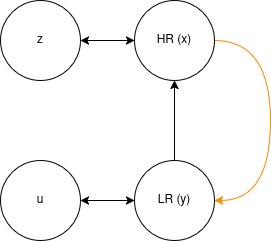
\includegraphics[width=0.5\linewidth]{img/SRVAE_deps.png}
    \caption{Graphique des dépendances variationnelles}
    \label{fig:vardeps}
\end{figure}

Expliquons les dépendances :
\definecolor{deporange}{RGB}{255, 88, 0}
\begin{itemize}
    \item u est la variable latente de y qui dépend directement d'y.
    \item z est la variable latente de x qui dépend directement d'x.
    \item y est une image sous-résolue de x, la \textcolor{deporange}{dépendance} d'y par rapport à x est considérée comme déterministe.
    \item x dépend de y étant sa version Haute Résolution, la transformation de y à x est "surjective" (plusieurs x pour un y donné).
\end{itemize}

\subsubsection{Simplifications}\label{simp}

Étant donné les dépendances vues plus tôt, nous allons nous autoriser plusieurs simplifications, notamment les suivantes :
\begin{itemize}
    \item $y|x$ déterministe.
    \item u ne dépend pas de x dans notre modèle. 
    \item $q(z|y,x,u) \approx q(z|x)$ soit z capture les informations contenues dans x qui ne sont pas dans y et u.
\end{itemize}
Pour le second point, nous considérons que les informations apportées par y sont suffisantes dans sa propre représentation. (Autrement dit, pas besoin de x pour la reconstruction de y, nous nous ramenons alors à un VAE classique).
De plus, nous n'avons pas accès à x dans un cas de super-résolution, donc nous ne pourrions pas l'utiliser hors de l'entrainement, donc ce qui poserait un problème pour sampler dans le modèle.

\subsubsection{Discussion}
Nous allons dans un premier temps développer les équations de la même manière que dans \cite{gatopoulos2020Superresolution}.

Il apparait évident que certaines simplifications sont potentiellement "optimistes". Nous pouvons notamment penser à enlever la dépendance en u pour reconstruire x. D'un premier point de vue, l'information est redondante avec y (u étant au mieux un changement de base de y, au pire une version compressée). Nous élaborerons les calculs avec puis sans cette simplification et nous observerons son effet sur les résultats.

\subsection{Évidence}
De la même manière que dans \ref{vae}, nous voulons maximiser $p(x)$. Commencons par poser $w = [u,z,y]$.
Avec notamment :
\begin{itemize}
    \item z, la variable latente de x
    \item y, la version basse résolution de x
    \item u, la variable latente de y
\end{itemize}

Nous pouvons donc exprimer $p(x)$ comme la marginalisation de la loi jointe de $(x,w)$. 
\begin{equation}
    p(x) = \int p(x,w)dw = \int \frac{p(x,w)}{q(w|x)}q(w|x)dw
\end{equation}

L'espérance conditionnelle est alors 
\begin{equation}
    p(x) = \mathbb{E}_{q(w|x)}\left[\frac{p(x,w)}{q(w|x)}\right]
\end{equation}

Commençons par réexprimer la loi jointe :
\begin{equation}
    p(x,w) = p(x|y,u,z)p(z|y,u)p(y|u)p(u)
\end{equation}

Nous pouvons négliger la dépendance en u pour x, car les informations sont redondantes avec y.
Cette loi jointe approximée est donc :
\begin{equation}
    p(x,w) \approx p(x|y,z)p(z|y,u)p(y|u)p(u)
\end{equation}

Nous avons également : 
\begin{equation}
     q(w|x) = q(z|y,x,u)q(u|x,y)q(y|x)
\end{equation}

Utilisant les simplifications de \ref{simp}, nous pouvons donc supprimer les dépendances "inutiles" dans $q(z|y,u,x)$
\begin{equation}
    q(w|x) \approx q(z|x)q(u|y)q(y|x)
\end{equation}

\subsection{Expression de la log-évidence}

En passant cette équation au log, nous pouvons donc exprimer l'évidence de la façon suivante, commençons par l'évidence :

\begin{equation*}
    p(x) = \mathbb{E}_{q(z|x)q(u|y)q(y|x)}\left[\frac{p(x|u,x,y)p(z|y,u)p(y|u)p(u)}{q(z|x)q(u|y)q(y|x)}\right]
\end{equation*}

En utilisant la formule de Jensen pour décomposer le terme de droite, nous pouvons obtenir l'inégalité suivante :
\begin{equation*}
    \log(p(x)) \geq \mathbb{E}_{q(z|x)q(u|y)q(y|x)}\left[\log\left(\frac{p(x|z,y)p(z|y,u)p(y|u)p(u)}{q(z|x)q(u|y)q(y|x)}\right)\right]
\end{equation*}

En développant les différents termes de cette équation, nous obtenons l'équation suivante que nous allons étudier termes par termes.

\begin{multline}
    \log(p(x)) \geq \mathbb{E}_{q(z|y,x)}\left[\log(p(x|y,z))\right] + \mathbb{E}_{q(z|y,x)q(u|y)}\left[\log(p(z|y,u))\right] \\+ \mathbb{E}_{q(u|y)}\left[\log(p(y|u))\right] + \mathbb{E}_{q(u|y)}\left[\log(p(u))\right] - \mathbb{E}_{q(z|x)q(u|y)}\left[\log(q(z|y,x))\right]\\ - \mathbb{E}_{q(u|y)}\left[\log(q(u|y))\right]
\end{multline}

\subsection{Attaches aux données}

Comme dans la section \ref{attdata}, nous pouvons sortir plusieurs termes d'attache aux données de cette équation, nous pouvons reconnaitre dès le début que :

\begin{align*}
    \mathcal{L}_x = \mathbb{E}_{q(z|y,x)}\left[\log(p(x|y,z))\right] && \mathcal{L}_y =\mathbb{E}_{q(u|y)}\left[\log(p(y|u))\right]
\end{align*}

Sont les deux termes d'attache aux données. Comme plus tôt, nous utilisons un décodeur à variance diagonale paramétrée par $\gamma_{x,y}$ qui sont deux variances apprises pour les deux décodeurs.

\subsubsection{Attache à y}

Cette partie est la plus simple car elle s'apparente le plus au VAE classique. En effet, nous avons donc un décodeur suivant la loi suivante :
\begin{equation}
    p(y|u) \sim \mathcal{N}(\mu_\theta, \gamma_y^2\mathbb{I})
\end{equation}

Développant cela, nous pouvons développer le terme $\mathcal{L}_y$ de la façon suivante
\begin{equation*}
    \mathcal{L}_y = \mathbb{E}_{q(z|y,x)}\left[-\frac{||y-\hat{y}||^2_2}{2\gamma_y^2} - N_y\log(\gamma_y) - \frac{N_y}{2}\log(2\pi) \right]  
\end{equation*}

Puisque nous ne pouvons pas optimiser le terme en $2\pi$, nous allons donc utiliser la proportionnalité pour optimiser le terme suivant :
\begin{equation}
    \mathcal{L}_y \propto -\mathbb{E}_{q(z|y,x)}\left[\frac{||y-\hat{y}||^2_2}{2\gamma_y^2}\right]  - N_y\log(\gamma_y)
\end{equation}

Cette espérance, ici, se calcule de façon empirique, nous obtenons alors les termes suivants :

\begin{equation*}
    \mathcal{L}_y \propto - \frac{N_y}{2 \gamma_y^2N_y}\sum_{i=1}^n(y_i-\hat{y}_i)^2   - N_y\log(\gamma_y) = -N_y \left[\frac{MSE(y,\hat{y})}{2\gamma_y^2} + log(\gamma_y)\right]
\end{equation*}

\subsubsection{Attache à x}

De la même façon que dans la sous-section précédente, nous pouvons développer le terme 

\begin{equation*}
    \mathcal{L}_x = \mathbb{E}_{q(z|y,x)}\left[\log(p(x|y,z))\right]
\end{equation*}

Cela nous donne alors :
\begin{equation*}
    \mathcal{L}_x \propto - \frac{N_x}{2 \gamma_x^2N_x}\sum_{i=1}^n(x_i-\hat{x}_i)^2   - N_x\log(\gamma_x) = -N_x \left[\frac{MSE(x,\hat{x})}{2\gamma_x^2} + log(\gamma_x)\right]
\end{equation*}

Un lecteur avisé se demandera, à juste titre, où est passée la dépendance en y dans ce terme. Ce terme en réalité se cache dans la loi du décodeur où nous avons en réalité :
\begin{equation}
    p(x|y,z) \sim \mathcal{N}(\mu_{\psi|y}, \gamma_x^2\mathbb{I})
\end{equation}
Le décodeur prend également y en entrée pour estimer x.

\subsection{Distance au priors}

De ce qu'il reste de non analysé dans l'ELBO, nous pouvons extraire plusieurs termes, qui sont, nous le verrons, des distances.
Ainsi, nous pouvons extraire les deux distances suivantes 
\begin{equation*}
 D_z = \mathbb{E}_{q(z|y,x)q(u|y)}\left[\log(p(z|y,u))\right]- \mathbb{E}_{q(z|y,x)q(u|y)}\left[\log(q(z|y,x))\right]
\end{equation*}
    
\begin{equation*}
 D_u = \mathbb{E}_{q(u|y)}\left[\log(p(u))\right] - \mathbb{E}_{q(u|y)}\left[\log(q(u|y))\right]
\end{equation*}

\subsubsection{Prior Gaussien}
Nous allons commencer par analyser $D_u$. Ce cas est relativement simple, car il s'agit, tout simplement, du VAE classique développé dans la section \ref{kl}.

\begin{equation*}
 D_u = \mathbb{E}_{q(u|y)}\left[\log\left(\frac{p(u)}{q(u|y)}\right)\right]
\end{equation*}

Par définition de l'espérance conditionnelle, nous avons donc en réalité :

\begin{equation*}
    D_u = - \int q(u|y) \log\left(\frac{q(u|y)}{p(u)}\right) = - \mathcal{KL}(q(u|y)||p(u)) 
\end{equation*}
On reconnait la divergence de Kullback-Leibler, la distance dont nous parlions plus tôt.

\subsubsection{Prior conditionnel}
Passons maintenant à la distance $D_z$ qui est moins évidente.
Le calcul se fait de la même façon et nous obtenons rapidement :
\begin{equation}
    D_z = - \mathcal{KL}(q(z|x)||p(z|y,u))
\end{equation}

La différence est donc que la prior de la branche Haute-Résolution n'est pas une gaussienne, mais une loi qui sera apprise.
Ne connaissant pas la loi, $z|y,u$ nous sommes donc obligés d'effectuer l'approximation par un réseau de neurones de la façon suivante :
\begin{equation*}
    p(z|y,u) \approx p_\phi(z|y,u)
\end{equation*}

\subsection{ELBO}
La négative ELBO (que l'on minimisera) s'exprime alors de façon très simple :

\begin{multline}
    - ELBO = N_y\left[\frac{MSE(y,\hat{y})}{2\gamma_y^2} + \log(\gamma_y)\right] + N_x\left[\frac{MSE(x,\hat{x})}{2\gamma_x^2} + \log(\gamma_x)\right]\\ + \mathcal{KL}(q(z|x)||p(z|y,u)) + \mathcal{KL}(q(u|y)||p(u)) 
\end{multline}

\subsection{Modèle plus complexe}
Plusieurs simplifications ont été faites dans le modèle précédent. Certaines sont judicieuses, d'autres, peut-être moins. Dans un cadre de super-résolution ou résolution d'un problème conditionnel, il est judicieux de supprimer la dépendance en x pour l'étage y quand nous voulons inférer x sachant y. C'est notre cas ici. Il peut notamment être intéressant de réinclure la dépendance en $u$ pour la reconstruction de $x$ de cette façon, nous pourrions propager les gradients de MSE dans les blocs de réseaux neuronaux qui s'occupent de la tâche de super-résolution. Cela devrait nous aider à améliorer les performances de la tâche en amont. L'implémentation est un problème d'architecture que nous n'étudierons pas ici.

Il peut également être intéressant d'étudier le rajout des dépendances en $y,u$ dans z.

\section{MoG}

Admettons maintenant un mélange de gaussiennes :
\begin{equation}
    p(u) = MoG(w, \mu, \sigma) = \sum_{i=1}^{Comp} w_i \mathcal{N}(\mu_i,\sigma_i^2)
\end{equation}

Nous ne changeons qu'une chose : le prior de u.
Qu'est ce que cela traduit pour l'ELBO ? 
Nous pouvons borner $\mathcal{KL}(p||\sum_i w_i q_i) \leq \sum_i w_i \mathcal{KL}(p||q_i)$. Ainsi, nous avons donc une borne inf de l'ELBO qui est une borne inf de $p(x)$.

Notre ELBO deviendrait alors :
\begin{multline}
    - ELBO = N_y\left[\frac{MSE(y,\hat{y})}{2\gamma_y^2} + \log(\gamma_y)\right] + N_x\left[\frac{MSE(x,\hat{x})}{2\gamma_x^2} + \log(\gamma_x)\right]\\ + \mathcal{KL}(q(z|x)||p(z|y,u)) + \sum_{i=1}^{n_w}w_i\mathcal{KL}(q(u|y)||p_i(u)) 
\end{multline}

Avec $p_i(u) \sim \mathcal{N}(\mu_i,\sigma_i^2)$.

\end{document}

